\chapter{T3b --- Muchos cuerpos: redes tensoriales}
\label{ch:t3b}

\ideacentral{T3b valida la vía \emph{complementaria} a muchos cuerpos: la misma
dinámica de relajación se captura con redes tensoriales (superket MPS) a coste
polinómico en la dimensión de enlace $\chi$, volviéndose \emph{exacta} al crecer
$\chi$ (error $\to10^{-7}$) y alcanzando $N=32$ ($4^{32}\approx10^{19}$, imposible
en denso). El parámetro $\chi$ ofrece un control sistemático de la precisión del
que las trayectorias (T3a) carecen.}

\section{Marco teórico}

La segunda vía para muchos cuerpos representa el operador densidad como una
\textbf{red tensorial}. En la representación vectorizada (Zwolak \& Vidal,
\emph{PRL} \textbf{93}, 207205, 2004), $\rho$ se escribe como un \emph{superket}
$\ket{\rho}\rangle$ que es un \emph{Matrix Product State} (MPS) con dimensión
física $4$ por sitio: el índice doblado $p=a\cdot2+b$ combina la fila $a$ y la
columna $b$ de cada qubit. La ecuación maestra se convierte en
\begin{equation}
    \frac{\dd}{\dd t}\ket{\rho}\rangle = \Lop\,\ket{\rho}\rangle,
\end{equation}
con $\Lop$ un operador local (suma de términos de $1$ y $2$ sitios). El coste de
representar y evolucionar el MPS es polinómico en la \emph{dimensión de enlace}
$\chi$, que controla el entrelazamiento (de operador) capturado. Si $\chi$ se
mantiene acotado, se alcanzan tamaños $N$ inaccesibles a cualquier método exacto.

\section{Método numérico: TEBD disipativo}

Se usa \textbf{TEBD} (Time-Evolving Block Decimation). El Liouvilliano se
descompone en generadores de \emph{bond} $\Lop=\sum_b \Lop_b$, asignando cada
término de un sitio a un bond adyacente para evitar doble conteo. La evolución
$e^{dt\Lop}$ se trotteriza con el esquema de Strang de segundo orden,
\begin{equation}
    e^{dt\Lop}\approx
    \Big(\!\!\prod_{b\,\text{par}}\! e^{\frac{dt}{2}\Lop_b}\Big)
    \Big(\!\!\prod_{b\,\text{impar}}\! e^{dt\Lop_b}\Big)
    \Big(\!\!\prod_{b\,\text{par}}\! e^{\frac{dt}{2}\Lop_b}\Big),
\end{equation}
donde cada compuerta $e^{dt\Lop_b}$ actúa sobre dos sitios contiguos del superket.
Tras aplicar una compuerta, el tensor conjunto se reseparaa por SVD y se
\emph{trunca} a los $\chi$ mayores valores singulares. Los generadores locales se
construyen reutilizando \texttt{common.qmpe.build\_liouvillian} (en base
\emph{column-stacking}) y permutando los índices al orden site-local $p=a\cdot2+b$;
la exponencial $e^{dt\Lop_b}$ se calcula por descomposición espectral de la matriz
$16\times16$. Los observables ($\Tr\rho$, densidad de excitación) se obtienen
contrayendo el MPS con los covectores $\langle\!\langle\mathbb{1}|$ y
$\langle\!\langle n_k|$.

\section{Implementación serial}

El núcleo serial está en \texttt{T3/T3b\_tensor\_networks/python/mpdo\_tebd.py}: la
clase \texttt{SuperketMPS} (tensores $(D_l,4,D_r)$) implementa la aplicación de
compuertas con truncación SVD, la traza y los valores esperados. La función
\texttt{evolve\_tebd} realiza la evolución de Strang completa.

\section{Justificación de la paralelización}

El paralelismo de TEBD es \emph{estructurado}: dentro de una capa de Trotter, las
compuertas sobre bonds \emph{disjuntos} ---los pares $(0,1),(2,3),\dots$ o los
impares $(1,2),(3,4),\dots$--- no comparten tensores y pueden aplicarse
simultáneamente. Cada compuerta realiza una SVD de coste $\mathcal{O}(\chi^3)$.
Como numpy libera el GIL durante la SVD/BLAS, se paralelizan con \emph{hilos}
(\texttt{ThreadPoolExecutor}) sin coste de serialización ---a diferencia de
\texttt{multiprocessing}, que requeriría copiar los tensores. Este patrón es
intermedio entre el SpMV acoplado de T1 y las trayectorias independientes de T3a.

\paragraph{Mapeo a memoria distribuida.} Para muchos nodos, el esquema se mapea a
MPI repartiendo segmentos contiguos de la cadena entre rangos, con intercambio de
los tensores de frontera por capa de Trotter; queda como trabajo futuro.

\section{Comparación y resultados}

\subsection{Validación y convergencia en $\chi$}

La \cref{fig:t3bval} valida el TEBD contra la ecuación maestra exacta (Ising
$N=4$): el error decae sistemáticamente al aumentar $\chi$,
\[
  6\times10^{-2}\ (\chi{=}1)\;\to\; 3\times10^{-3}\ (\chi{=}4)\;\to\;
  6.3\times10^{-7}\ (\chi{=}16),
\]
alcanzando precisión esencialmente exacta cuando $\chi$ iguala el rango máximo del
sistema ($\chi=16$ para $N=4$). Esto confirma la correctitud del esquema de
índices y de la truncación.

\begin{figure}[t]
\centering
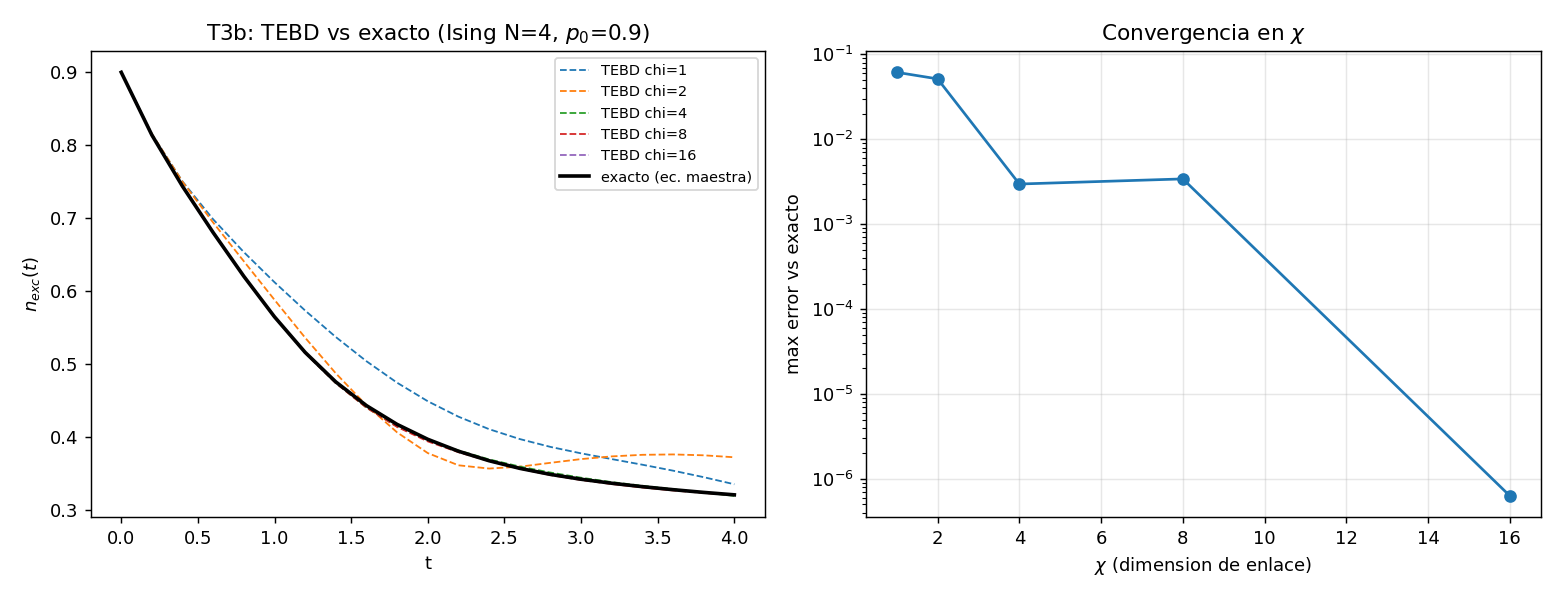
\includegraphics[width=\textwidth]{figures/t3b_validation.png}
\caption{T3b: (izq.) densidad de excitación, TEBD a distintos $\chi$ frente al
exacto (Ising $N=4$); (der.) error máximo frente a $\chi$ (escala log).}
\label{fig:t3bval}
\end{figure}

\subsection{Escalado y muchos cuerpos}

La \cref{fig:t3bscaling} muestra el escalado del TEBD paralelo por compuertas
(Ising $N=20$, $\chi=48$, con BLAS de un hilo para aislar el paralelismo): $1.84\times$
(2 hilos), $2.72\times$ (4) y $3.61\times$ (8). El escalado es bueno pero no ideal:
el número de bonds disjuntos por capa ($\sim N/2$) y el desbalance de carga (los
tensores centrales alcanzan mayor $\chi$ que los de los extremos) limitan la
eficiencia, ilustrando el paralelismo estructurado con granularidad media.

\begin{table}[h]
\centering
\caption{T3b: speedup del TEBD paralelo por compuertas (Ising $N=20$, $\chi=48$).}
\label{tab:t3bscaling}
\begin{tabular}{cc}
\toprule
hilos & speedup \\
\midrule
2 & $1.84\times$ \\
4 & $2.72\times$ \\
8 & $3.61\times$ \\
\bottomrule
\end{tabular}
\end{table}

\begin{figure}[t]
\centering
\begin{subfigure}{0.49\textwidth}
  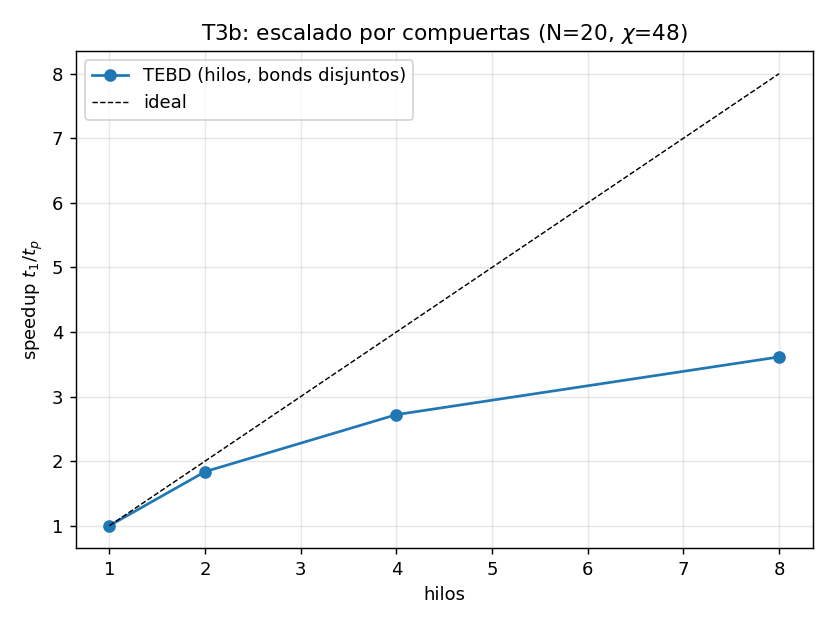
\includegraphics[width=\textwidth]{figures/t3b_scaling.png}
\end{subfigure}\hfill
\begin{subfigure}{0.49\textwidth}
  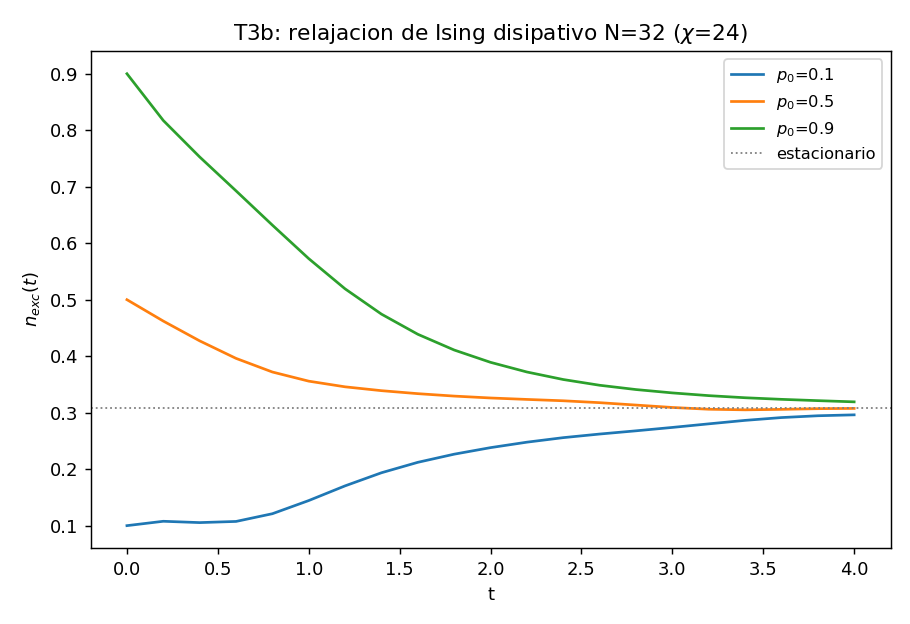
\includegraphics[width=\textwidth]{figures/t3b_largeN.png}
\end{subfigure}
\caption{T3b: (izq.) escalado por compuertas (N=20, $\chi=48$); (der.) relajación
de la cadena de Ising disipativa con $N=32$ sitios ($4^{32}\approx1.8\times10^{19}$,
imposible en denso), evolucionada con $\chi=24$ en $\sim3.6$\,s.}
\label{fig:t3bscaling}
\end{figure}

La demostración de muchos cuerpos evoluciona $N=32$ sitios ---cuyo Liouvilliano
denso tendría dimensión $4^{32}\approx1.8\times10^{19}$, absolutamente
inalcanzable--- con $\chi=24$ en unos $3.6$\,s por preparación. Las tres
preparaciones ($p_0=0.1,0.5,0.9$) relajan hacia un estacionario común, mostrando
que la red tensorial captura la dinámica de relajación con recursos polinómicos.
